% This is based on the LLNCS.DEM the demonstration file of
% the LaTeX macro package from Springer-Verlag
% for Lecture Notes in Computer Science,
% version 2.4 for LaTeX2e as of 16. April 2010
%
% See http://www.springer.com/computer/lncs/lncs+authors?SGWID=0-40209-0-0-0
% for the full guidelines.
%

\documentclass{llncs}
\usepackage{float}
\usepackage{graphicx}
\usepackage{hyperref}
\usepackage{cleveref}
\usepackage{xepersian}
\usepackage{setspace}
\settextfont[Scale=1.2]{XWZar.ttf}
\setlatintextfont[Scale=1]{Times New Roman}
\pagestyle{plain}



\newcommand{\quotes}[1]{``#1''}
\doublespacing
\begin{document}

\title{گزارش کاراموزی}
%
%

\author{محمدمهدی رحیمی \\  \\ استاد کارآموزی: \\ جعفر عبدی \\  \\ \\ استاد در صنعت: \\ سهند دادخواه فر}

\maketitle              % typeset the title of the contribution

\begin{figure}[h]
\centering

\includegraphics[width=0.3\textwidth]{mahi/AUT_logo.png}
\centering
\label{fig:aut}
\end{figure}
\newpage
\title{\begin{center}
\begin{normalsize}
\textbf{چکیده} 
\end{normalsize}
\end{center} }
\begin{abstract}
در این گزارش ابتدا به هوش تجاری و مفاهیم پایه آن مورد بررسی قرار میگیرد، سپس راه حل و نحوه پیاده سازی آن برای شرکت ها مخابراتی و استاندارد ها جهانی آن توصیف میشود.
در ادامه راهکار پیاده سازی شده توسط شرکت پرتوآبی برای اپراتور همراه اول شرح داده میشود و در انتها پروژه مانیتورینگ بلادرنگ سیستم با جزییات شرح داده میشود.
\\
\\
\textbf{کلمات کلیدی:} هوش تجاری، کلان داده ها، پردازش بلادرنگ، سیستم های مانیتورینگ

\end{abstract}
\newpage
%
\tableofcontents
\newpage
\listoffigures
\newpage
\addtocontents{toc}{\setcounter{tocdepth}{1}}
\section{مقدمه}
هوش تجاری به بررسی دقیق و کامل در مورد تمامی درآمد ها و هزینه های هر سازمان و شرکت با استفاده از تمامی داده ها تولید شده از بخش های مختلف آن سازمان میپردازد.
نتایج این بررسی معمولا در قالب داشپور و یا گزارش های روزانه برای قسمت ها مدیریت، بازاریابی و یا اداره ها مربوط در دسترس قرار میگیرد.
در این سیستم یکپارچگی و صحت داده ها در کنار قابل دسترس بودن و قابل اطمینان بودن آن به شدت مهم است.
از آن جا که حجم داده های ورودی به شدت بالا میباشد این سیستم باید بتواند به صورت بلادرنگ داده ها را پردازش کند و سرعت اجرای پردازش و جلوگیری و رفع خطا در پردازش بخشی از نیازمندی های اساسی این پروژه شمرده میشود.
از این رو در کتار این سیستم پردازشی به یک سیستم مانیتورینگ بلادرنگ نیز احتیاج است تا بتوان در اولین فرصت مشکلات را تشخیص داد و حل کرد و در صورت امکان از بروز مشکلات جلوگیری شود.
در این گزارش بعد از معرفی سیستم و عملکرد آن به بررسی نحوه پیاده سازی و اجرای سیستم مانیتورینگ که توسط کارآموز به طور کامل راه اندازی شده است میپردازد.
\newpage
\section {هوش تجاری}
\addtocontents{toc}{\setcounter{tocdepth}{2}}
\subsection{مقدمه بر هوش تجاری}
فناوری‌های نوین با سرعتی سرسام آور در حال پیشرفت هستند، بطوریکه جوامع بصورت عام و بازار بصورت خاص با شتابی وصف‌ناپذیر بدنبال ترفندهایی می‌گردند که بقایشان را در این عرصه آشفته و متلاطم تضمین کنند. سازمانها باید بپذیرند که فلسفه حیاتشان تغییر کرده است و دیگر زنده بودن به معنای رسیدن به وضعیت سوددهی مداوم نمی‌تواند باشد و باید بدنبال رقابت و ابزار آن باشند،

چرا که امروزه کمتر شرکتی در این عرصه بصورت سنتی و به دور از قواعد جدید بازی کسب و کار، به تلاش ادامه می‌دهد و برای اینکه بتوان پابه‌پای رقبا باقی ماند یا شاید بسختی و با مهارت بسیار بتوان یک قدم از آنها پیش گرفت، می‌بایست به قواعد جدید بازی کاملا مسلط بود تا شاید روزی بتوان خود را یک قاعده جدید انگاشت.

بنابراین تسلط بر فناوری‌های جدیدی مانند هوش تجاری در کسب و کارها یک الزام و ضرورتی اجتناب ناپذیر تلقی می‌شود. هدف نیز چیزی جز یادآوری روند روبه رشد و توقف‌ناپذیر نوآوری در فناوری و دگرگونی در نحوه کسب و کارها نیست. تحولی که در این انقلاب صورت پذیرفته است و دگرگونی‌هایی که در رویه تغییرات موجبات بروز اختلافات و پیدایش شکاف‌های عمیقی را بین فرداها با امروز فراهم آورده و خواهد آورد.

هوش تجاری، Business Intelligence یا به اختصار BI یک فرآیند تکنولوژی محور برای تحلیل داده هاست. این فرآیند در نهایت به مدیران، صاحبان کسب و کار و تمام تصمیم گیرنده‌های اساسی یک کسب و کار، اطلاعاتی عملی می‌دهد. ابزارهای BI برای آنالیز و تحلیل داده‌ها به صورت‌های مختلفی ارائه می‌شود؛ مثلا گزارش، داشبورد، چارت، نقشه، گراف و تمام ابزارهایی که بتوانند اطلاعات و داده‌های خام را در قالب‌های بصری و قابل استفاده به نمایش درآورند.

در حقیقت هوش تجاری به شما به عنوان یک مدیر کمک می‌کند، بفهمید که چه عواملی در موفقیت یا شکست پروژه‌هایتان موثر است. همین باعث می‌شود که بتوانید بفهمید چه عواملی سود بیشتر برای شما رقم می‌زنند و چه عواملی سود کمتری برای شما به همراه دارند.

BI طیف گسترده‌ای از ابزار، اپلیکیشن‌ و متدلوژی را شامل می‌شود که به یک سازمان کمک می‌کند که بتواند اطلاعات (Data) را از سیستم داخلی و منابع خارجی شرکت جمع‌آوری کند و آنها را برای تحلیل آماده کند. از مجموع این اطلاعات در نهایت یک گزارش تهیه می‌شود که به مدیر و تصمیم گیرنده نهایی سازمان تحویل داده می‌شود. اجازه بدهید با یک مثال این لقمۀ قلمنبه سلنبه را برایتان به راحت الحلقوم تبدیل کنم.


\subsection{هوش تجاری چیست؟}
تعاریف زیادی برای هوش تجاری وجود دارد، اما بطورکلی هوش تجاری بعنوان یک رویکرد جدید در معماری سازمانی مطرح شده است که این معماری براساس سرعت در تحلیل اطلاعات به مدیران جهت اتخاذ تصمیمات دقیق و هوشمند کسب و کار در حداقل زمان ممکن کمک می‌کند. هوش تجاری یک چارچوب کاری شامل فرایندها، ابزار و فناوری‌های مختلف است که برای تبدیل داده به اطلاعات و اطلاعات به دانش مورد نیاز هستند، که با استفاده از همین دانش مدیران قادر به تصمیم‌گیری بهتر می‌شوند و در نتیجه عملکرد سازمان خود را بهبود می‌بخشند.

\begin{figure}
\centering
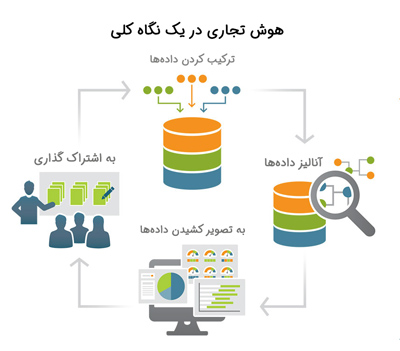
\includegraphics[width=0.75\textwidth]{mahi/bi-1.jpg}
\centering
\caption{هوش تجاری در یک نگاه}
\label{fig:bi-1}
\end{figure}


با پیاده‌سازی راهکارهای هوش تجاری فاصله موجود بین مدیران میانی و مدیران ارشد از دیدگاه ارتباط اطلاعاتی از میان خواهد رفت و اطلاعات مورد نیاز مدیران در هر سطح، در لحظه و با کیفیت بالا در اختیار آنها قرار خواهد گرفت. همچنین کارشناسان و تحلیل‌گران می‌توانند با استفاده از امکانات ساده، فعالیتهای خود را بهبود بخشند و به نتایج بهتری دست پیدا نمایند.

\textbf{ارزش مدیریت در تصمیم گیری صحیح و به موقع است}
احساس نیاز به وجود یک سیستم هوش تجاری در سازمان برای اولین بار در سطوح بالای مدیریتی احساس می‌شود و از بالای هرم ساختار سازمانی به بخش‌های زیرین منتقل می‌گردد. مهم‌ترین نیاز یک مدیر، تصمیم‌گیری است. فرآیند تصمیم‌گیری می‌تواند به سه بخش کلی تقسیم شود که عبارتند از:
\begin{enumerate}
    \item دسترسی،جمع‌آوری و پالایش داده ها و اطلاعات موردنیاز
    \item پردازش، تحلیل و نتیجه گیری بر اساس دانش
    \item اعمال نتیجه و نظارت بر پیامدهای اجرای آن
\end{enumerate}
در هر یک از موارد فوق، سازمانهای قدیمی که از هوش تجاری استفاده نمی‌کنند، دارای مشکلاتی هستند که اغلب از عواملی چون حجیم بودن داده‌ها، پیچیدگی در تحلیلها و ناتوانی در ردگیری نتایج فرایندها و پیامدهای تصمیمات گرفته شده، نشات می‌گیرند. هوش تجاری با کمک به حل مشکلات فوق، بدلیل ساختاری که در سازمان به وجود می‌آورد، فرصتهای جدیدی نیز برای رشد سازمان ایجاد می‌کند و نه تنها عامل حذف مشکلات است، بلکه با صرفه‌جویی در زمان و هزینه، شرایط کاری را دگرگون می‌سازد.

\subsection{مراحل استقرار هوش تجاری}
هوش تجاری چارچوبی شامل فرآیندها، ابزار و فناوری مختلف است.
\begin{enumerate}
    \item منابع داده در مرحله اول جمع‌آوری می‌شوند. این منابع می‌تواند داده‌های انواع پایگاه داده یا اطلاعات نرم‌افزارهای موجود را در بر بگیرد.
    \item اطلاعات جمع‌آوری شده طی فرایند ETL در پایگاه داده تحلیلی یا همان انبار داده بارگذاری می‌شود.
    \item داده در پایگاه داده تحلیلی در بخش‌های مجزایی به نام داده گاه قرار می‌گیرد.
    \item در مرحله بعد هوش تجاری وارد عمل شده و روی اطلاعات طبقه‌بندی شده تجزیه و تحلیل انجام می‌دهد.
    \item در نهایت اطلاعات جهت انتشار به ابزارهای سطح بالا تحویل داده می‌شود.

\end{enumerate}

\begin{figure}
\centering
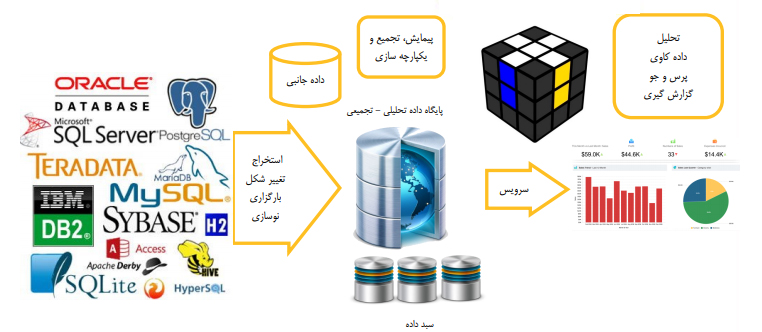
\includegraphics[width=0.5\textwidth]{mahi/bi-2.jpg}
\centering
\caption{معماری هوش تجاری با نمایش ابزار}
\label{fig:bi-2}
\end{figure}
\begin{figure}
\centering
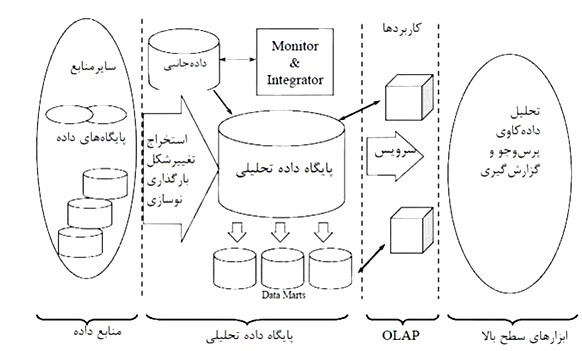
\includegraphics[width=0.5\textwidth]{mahi/bi-3.jpg}
\centering
\caption{معماری هوش تجاری به صورت منطقی}
\label{fig:bi-3}
\end{figure}

\subsection{گلیات هوش تجاری}
هوش تجاری یا هوش کسب و کار که قالب عمده‌تری را مانند استفاده‌های تجاری و غیر تجاری (نظامی و غیر‌انتفاعی) در بر دارد، عبارت است از بُعد وسیعی از کاربردها و تکنولوژی برای جمع‌آوری داده و دانش جهت زایش پرس و جو در راستای آنالیز بنگاه برای اتخاذ تصمیمات تجاری دقیق و هوشمند.

یک هوش تجاری براساس یک معماری بنگاه تشکیل شده است و در قالب پردازش تحلیلی برخط به تحلیل داده‌های تجاری و اتخاذ تصمیمات دقیق و هوشمند می‌پردازد. هوش تجاری، نه بعنوان یک محصول و نه بعنوان یک سیستم، بلکه بعنوان یک معماری و رویکردی جدید موردنظر است. که البته شامل مجموعه‌ای از برنامه‌های کاربردی و تحلیلی است که به استناد پایگاه‌های داده عملیاتی و تحلیلی به اخذ و کمک به تصمیم‌گیری برای فعالیت‌های هوشمند تجاری و کسب و کار می‌پردازند.

\subsection{هوش تجاری از مناظر دیگر}
\begin{enumerate}
    \item از منظر معماری و فرایند به هوش تجاری به عنوان یک چارچوب که عامل افزایش کارایی سازمان و یکپارچگی فرایندها و نهایتا بر فرایندهای تصمیم‌گیری در سطوح مختلف سازمانی متمرکز است، نگریسته می‌شود.
    \item بازار هوش تجاری را ابزاری برای برتری رقابتی و پایشگر و تحلیلگر بازار و مشتریان می‌داند.
    \item از نقطه نظر فناوری نیز هوش تجاری یک سیستم هوشمند است که با پردازش دقیق داده‌ها، نقطه دخالت سخت افزار و نرم افزار در مغز افزارها به حساب می‌آید.
    \item ولی به بیان ساده‌تر هوش تجاری چیزی نیست مگر فرایند بالابردن سوددهی سازمان در بازار رقابتی با استفاده هوشمندانه از داده‌های موجود در فرایند تصمیم‌گیری.
\end{enumerate}
در صورتیکه مفهوم هوش تجاری بدرستی درک و منتقل نگردد، موجب می‌شود تا انتظارات مدیران به صورت ناگهانی افزایش یابد و برآورده نشدن این توقعات مواردی را از جمله سلب اطمینان افراد و بویژه مدیران از این سیستم به دنبال خواهد داشت. چرا که هوش تجاری فقط به دنبال کوتاه کردن مسیرهای پرس‌وجو در داخل اطلاعات است و خود مستقلا و بدون نیاز به اطلاعات مناسب قادر به ارائه پیشنهاد یا راهکاری نیست.

\subsection{تفاوت BI و BA}
BA مخفف عبارت Business Analytics است. BA از ابزارهای تحلیل داده کمک می‌گیرد تا بتواند پیش‌بینی کند که چه اتفاقی برای آیندۀ کسب و کار می‌افتد. در حقیقت BI بیشتر به یک فرآیند اشاره می‌کند که داده‌ها را برای ما فراهم می‌کند. اما BA بیشتر به یک شخص اشاره می‌کند که بر مبنای این اطلاعات راه‌حل برای بیزینس پیدا می‌کند. در حقیقت می‌توانیم اینطور بگوییم که BA یکی از اجزای فرآیند BI حساب می‌شود.
به نظر می‌رسد که حالا تا حدودی با کلیت هوش تجاری آشنا شده‌اید. اما BI دقیقا چه فوایدی برای کسب و کار شما دارد؟


\subsection{مزایا استفاده از هوش تجاری}
\begin{enumerate}
  \item \textit{راحتی در تهیه گزارش}
  \newline
هر شرکت یا کسب و کاری بخش‌ها و دپارتمان‌های متفاوتی دارد. اطلاعات بخش‌های مختلف در فرمت‌های مختلف پخش شده‌اند. بیشتر تلاش‌هایی که برای جمع‌آوری اطلاعات انجام می‌شود، باید این اطلاعات را مرتب کند و به فرمتی تبدیل کند که بتوان آنها را تحلیل و بررسی کرد. با استفاده از ابزارهای پیشرفتۀ هوش تجاری در کمترین زمان ممکن می‌تواند یک گزارش کامل و خوانا از هرکدام از بخش‌های شرکت داشته باشید.

به عنوان یک مدیر یا صاحب کسب و کار، این برای شما کاملا حیاتی است که بدانید که دیتاهای شرکت شما به شما چه می‌گویند. البته واضح است که اطلاعات معادل هوش نیست. این مخصوص به زمانی است فوق‌العاده کاربرد دارد که شرکت شما بخش‌های مختلف دارد و اطالاعات بخش‌های مختلف چندان به هم مرتبط نیستند و شما برای تصمیم‌گیری به این اطلاعات نیاز دارید.

  \item \textit{تصمیم گیری سریع و هوشمندانه}
  \newline
بگذارید اینطور برایتان بگویم، تمام درآمد و سود شرکت مستقیما به تصمیمات استراتژیک مربوط می‌شود.

شاید برایتان جالب باشد بدانید که مدت زمان تقریبی برای برای تهیه یک گزارش IT چیزی حدود دو روز است. در جهان پر سرعت معاصر، داده‌ها مدام در حال تغییر و نوسان هستند. در طول دو روز داده‌ها تغییرات زیادی می‌کنند. در حقیقت مدیران و استراتژیست‌های شرکت نیاز دارند که به اطلاعات به روز (آپدیت) دسترسی داشته باشند تا بتوانند به سرعت تصمیم بگیرند و جایگاه خود را در بازار از دست ندهند.

این اعداد و ارقام اصلا چیز کمی نیستند، دقیقا به کمک همین اعداد و ارقام است که می‌توانید راه‌حل‌های درست و درآمدزا برای کسب و کار خود پیدا کنید.

هدف نهایی یک کارشناس BI این است که اطلاعات شرکت شما را به یک تجزیه تحلیل ساختارمند تبدیل کند. به بیانی دیگر یک کارشناس واقعی هوش تجاری که می‌تواند به تصمیمات استراتژیک و سریع شرکت کمک کند.

هوش تجاری با اطلاعات به روزی که در اختیار مدیران قرار می‌دهد کمک می‌کند که وضعیت مالی شرکت به سمت مثبت حرکت کنید و تصمیمات درست گرفته شود.

  \item \textit{بالا بردن بهره‌وری}
  \newline
هوش تجاری این قابلیت را دارد که راهکارهای نادرست را مشخص کند، وضع کنونی شرکت را به دقت مشخص کند و در ادامه مشخص کند که روزانه چه کارهایی باید انجام شود، اولویت‌های شرکت چیست و هرکس چه کاری باید انجام دهد. در حقیقت قرار است ببیند که در کدام بخش‌ها ضعف وجود دارد،کدام بخش‌ها باید پیشرفت کنند و به امکانات جدیدتری مجهز شوند.

شاید برایتان جالب باشد بدانید بر اساس آمار سال 2000 سایت CIO شرکت تویوتا با استفاده از ابزارهای هوش تجاری توانست بفهمد که در فرآیند توزیع و تحویل کالا نیمی از هزینه بیش ازآنچیزی است که باید باشد و با تغییر استراتژی این هزینه را 50\% کاهش داد.

  \item \textit{سرعت بخشیدن به بازگشت سرمایه}
    \newline
اوج تمام خواسته‌های یک شرکت و تمام چیزهایی که در بالا گفتیم می‌تواند در "رشد سریع برای بازگشت سرمایه" خلاصه شود. بدون بینش درست و دیسیپلین مشخص، یا در در دام روش‌های نخ‌نما و قدیمی می‌افتید یا به حدس و گمانه‌زنی در مورد رفتارهای کاربران و چیزهایی از این قبیل می‌افتید. این‌ها مهم‌ترین آفت‌های کسب و کار شما هستند و دقیقا همان چیزهایی هستند که باعث شکست کسب و کار شما و بسیاری دیگر مانند شما می‌شوند.

همانطور که قبلا هم اشاره کردیم، هر شرکت یک سیستم است که تمام بخش‌های آن به نوعی با هم مرتبط هستند و نمی‌شود که برای هر بخش آن یک استراتژی جداگانه ریخت و به بقیۀ بخش‌ها کاری نداشت. تمام تلاش هوش تجاری این است که اطلاعاتی ارائه دهد که اگر چه برای هر بخش به طور جداگانه موجود است، اما بتواند یک کلیتی به ما بدهد که بر مبنای آن تصمیم‌گیری کرد، استراتزی چید و برنامه عملی ریخت.

دقیقا به همین دلیل است که BI می‌تواند به روشنی به شما کمک کند که کمپین‌های خود را برنامه‌ریزی کنید و هر چیزی را که لازم است تغییر دهید، تغییر دهید پیش از آنکه واقعا دیر شود و در کمترین زمان ممکن سرمایه شما را به شما بازمی‌گرداند.

  \item \textit{کاهش هزینه نیرو انسانی}
  \newline
با رشد و پیشرفت جهان امروز ما، مهم‌ترین نیازی که جهان کسب و کار از هر زمان دیگری بیشتر به آن نیاز دارد، نیاز به تجزیه تحلیل داده‌ها و اطلاعات است. از طرف دیگر خود این داده‌ها روز به روز پیچیده‌تر و چند بعدی‌تر می‌شوند، چراکه شرکت‌ها و کسب و کارها مدام در حرکت به سوی گسترده‌شدن و توسغه حرکت می‌کنند. پس به موازات این حرکت نیاز به نیروهای انسانی متخصص برای تحلیل داده‌ها و تهیه گزارشات هم از هر زمان دیگری بیشتر می‌شود. اگر بخواهید از روش‌های سنتی استفاده کنید باید تعداد زیادی نیرو استخدام کنید، مدام گزارش بخواهید و مدام کسی باشد که این گزارشات را چک کند، اما یک متخصص هوش تجاری تمام اینکارها را انجام می‌دهد و در سریع‌ترین زمان ممکن گزارشات مورد نیاز شما را تهیه می‌کند. به عبارتی دیگر در وقت، زمان و هزینۀ شما به شدت صرفه‌جویی می‌کند.

\end{enumerate}

\subsection{ابعاد هوش تجاری}
\begin{enumerate}
\item \textbf{بعد فنی}
\newline

اساس بعد فنی یا تکنیکال به بخش ساخت انباره داده و عملیات مربوط به دیتابیس، انتقال داده، ابزارهای داشبوردساز و مکعب های اطلاعاتی یا Cube مربوط می‌شود. (در مورد این مکعب‌های اطلاعاتی در مقالات آینده به تفصیل صحبت خواهیم کرد)

این اولین، مهم‌ترین و در عین حال ساده‌ترین بخش هوش تجاری است. اگر بخواهم به زبان ساده این مرحله را تشریح کنم، باید بگویم که این بخش سه مرحلۀ اصلی دارد:

شناخت: در مرحله اول شما باید یک تحلیل جامع از کسب و کار داشته باشید، وضعیت موجود را بسنجید و بخش‌های مختلف آن را شناسایی کنید.
طراحی انبار داده: در این مرحله بر اساس اطلاعاتی که در مرحله قبل بدست آوردید، باید یک انبار داده یا Data Warehouse بسازید.
تهیه گزارش: در آخرین مرحلۀ این بخش که تهیه گزارش است، شما بر اساس انبار داده‌های خود گزارش تهیه می‌کنید و اطلاعات خام را به اطلاعات قابل فهم تبدیل می‌کنید.
مثلا وقتی یک خرید اینترنتی انجام می‌شود، در دیتابیس اطلاعاتی نظیر تاریخ، ساعت، شناسۀ مشتری ، کالای خریداری شده، تامین کنندۀ کالا، تعداد و قیمت خرید و فروش و این قبیل اطلاعات باید در سیستم ثبت شود.

در نهایت از این دیتابیس داشبوردهای مدیریتی و خلاصه شده ساخته می‌شود؛ مثلا اینکه امروز، این هفته یا این ماه چقدر سود داشتیم، مقدار این سود نسبت به سال قبل چقدر تغییر داشته، از ماه قبل تا این ماه چند مشتری جدید اضافه شدند و ....

\item \textbf{بعد فرهنگی}
\newline
بعد فرهنگی هوش تجاری به آنالیز درست نیازمندی‌ها، فرهنگ استفاده و تفکر مربوط می‌شود. در حقیقت در این بخش تصیمم‌گیری بر مبنای واقعیت‌های موجود (داده‌ها) انجام می‌شود. این مرحله به زیرساخت‌های رفتاری اساسی نیاز است که متاسفانه بیشتر موارد آن در ایران وجود ندارد. برای اینکه این بخش به خوبی انجام شود به نقد و تغییر پذیری مداوم ، انعطاف سازمانی بالا و اینرسی (مقاومت) سازمانی پایین در قبال تغییرات لازم است.

برای اینکه با این داشبوردها و گزارشات آشنا شوید، یک تصویر برایتان می‌آورم که ببینید چگونه یک گزارش خوب هوش تجاری در کمتر از یک دقیقه می‌تواند مهم‌ترین اطلاعاتی که یک مدیر لازم دارد را به او بدهد.

\end{enumerate}

\newpage

\section{استاندارد و مدل ITDM}
\subsection{ITDM چیست؟}
ITDM یا به عبارت دیگر Intellica Telecommunication Data Model یک مدل برای تجارت در صنعت مخابرات در سطح جهانی است. این مدل ساختار یافته، جامع و قابل توسعه است که به راختی میتوان از آن استفاده کرد و یا توسعه پیدا کند.

\subsection{ITDM برای چیست؟}
\begin{enumerate}
    \item دخیره سازی داده ها با بیشترین حد از جزییات
    \item حذف تکرار داده ها با نرمال سازی
    \item ذخیره داده ها با مدل طبیعی کسپ و کار
    \item مناسب برای اجرا آنالیز های پیچیده و پیدا کردن روابط بین داده ها
\end{enumerate}


\begin{figure}
\centering
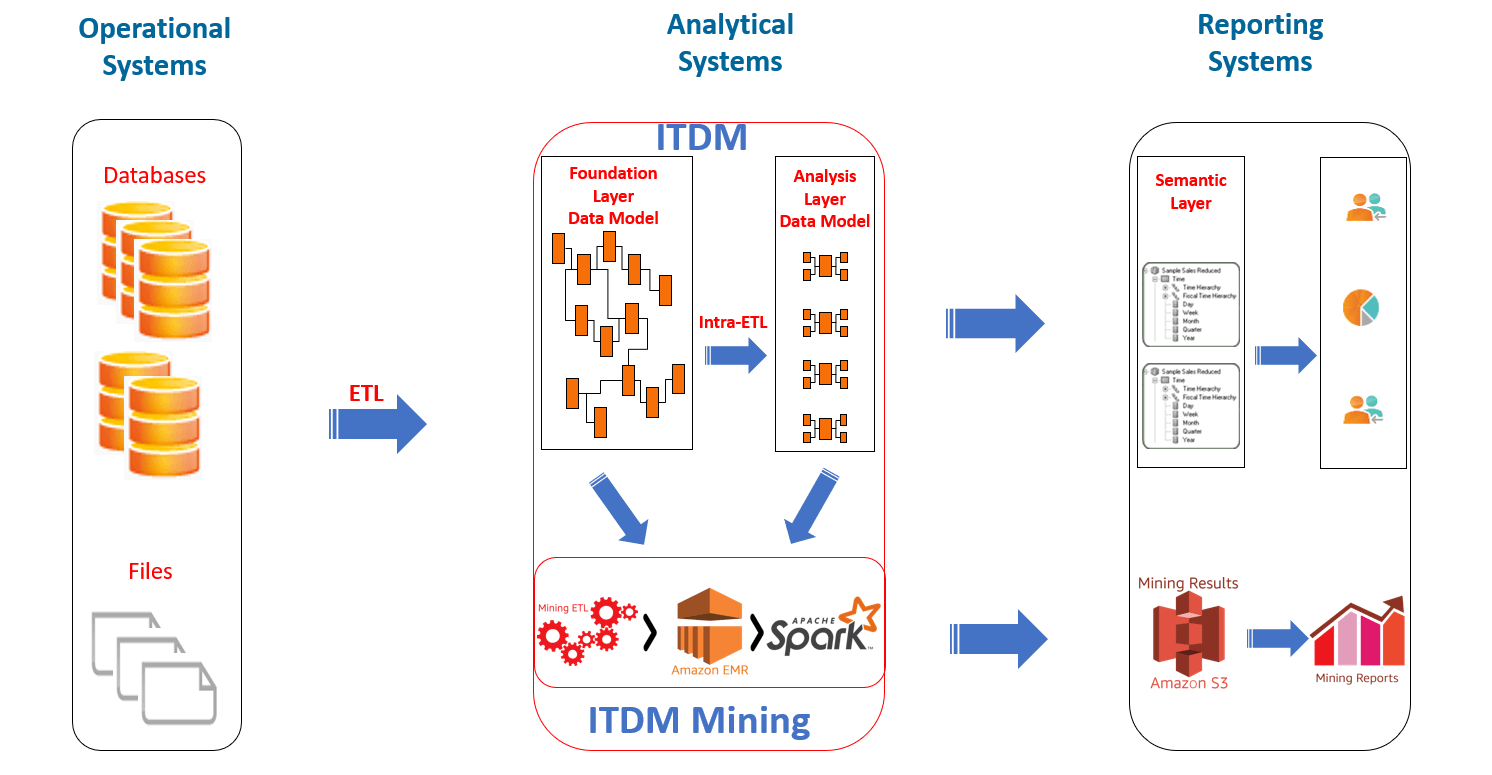
\includegraphics[width=1\textwidth]{mahi/bi-4.png}
\centering
\caption{معماری و مدل ITDM}
\label{fig:bi-4}
\end{figure}

\newpage

\subsection{آنالیز های پوشش داده شده از مخاربرات}
\begin{enumerate}
    \item Account Payment \& Adjustment
    \item Agreement
    \item Billing \& Invoice
    \item Campaign History
    \item Commission
    \item Commitment
    \item Contact Center
    \item Cost Center
    \item Customer Network Experience
    \item Customer Order
    \item Customer Churn
    \item Data Usage \& DPI
    \item Debt \& Collection
    \item Dunning
    \item Interconnect
    \item Inventory
    \item Market Share
    \item Operator Settlement
    \item Prepaid Recharge
    \item Revenue
    \item Roaming
    \item Sales
    \item Social Network
    \item Subscription
    \item Subscription Base Summary
    \item Traffic
    \item VAS
\end{enumerate}


\section {راهکار و ابزار ها}
\subsection{معماری پروژه }
معماری این پروژه به طور کلی به دو بخش dataware-house و analysis area تقسیم میشود.

\subsubsection{Dataware House}
این قسمت از پروژه به جمع آوری داده ها و نگه داری آن میپردازد.
جمع آوری داده ها میتواند از طریق فایل، ارتیاط مستقیم با پایگاه داده، ارتباط مستقیم از طریق شبکه و یا اتصال به نرم افزار های از طریق API آنها میباشد.

در مرحله اول جمع اوری داده ها تمامی اطلاعات بدون فیلتر و یا تغییر فقط در قابل استاندارد و ساختار یافته وارد پایگاه داده میشود.
با توجه به اندازه پروژه و داده ها پایگاه داده Oracle مورد استفاده قرار گرفته است که بر روی سرور های M10 و سیستم عامل Solaris Sparc که برای چنین پایگاه داده هایی بهینه سازی شده است استفاده میشود.
برای نگه داری این پایگاه داده تیمی متشکل از ده نفر برای بخش های شبکه، سیستم عامل، زیرساخت پایگاه داده و مدیریت پایگاه داده وجود دارد تا به صورت شبانه روزی تمامی تغییرات مانیتور شود و در صورت نیاز راهکار های جدید پیاده سازی شود.
تمامی تغییرات ساختاری و پایه ای بر روی پایگاه داده تنها توسط این افراد بر روی سیستم اعمال میشود.

\subsection{Foundation}
در این لایه از نرم‌افزار داده ها دریافتی که بدون فیلتر و تغییر در پایگاه داده قرار گرفته بودند، مورد ارزیابی قرار میگیرد و داده های معتبر و صجیج از نظر محتوایی به این لایه انتقال پیدا میکنند.
علاوه بر فیلتر داده و حذف داده های نامعتبر در این لایه از پایگاه داده ارتباط بین جداول و اشیا با استفاده از کلید های خارجی مشخص میشود.
به علت حجم کلان داده ها کلید خارجی و اولیه به صورت منطقی برای نرم‌افزار تعریف شده است و چنین شرط هایی در لایه پایگاه داده تعریف و پیاده سازی نمیشود، زیرا سرعت لود داده ها و تغییر آنها به شدت کاهش پیدا میکند و سیستم از حالت بلادرنگ خارج میشود.

در این قسمت طیق استاندارد ITDM تمامی رکورد های در پایگاه داده قالب مشخص خود را میگیرد و ارتباط های بین داده ها و تراکنش ها با مشتریان تماما مشخص میشود.



\subsection{Analysis Area}
در این لایه داده ها طوری پردازش میشود که مورد استفاده مستقیم برای داشبورد ها و گزارش ها قرار گیرد.
تمامی پردازش داده ها و تحلیل ها در این بخش صورت میگیرد، و نیازمندی های این بخش توسط KPI ها تعریف و اندازه گیری میشود.
این لایه از نرم‌افزار ممکن است بارها تغییر کند و پردازش شود تا به نتیجه صحیح برسد اما نیازی به ایجاد تغییر در لایه های پایین برای اصلاح تحلیل ها نیست.


\subsection{سیستم گزارش دهی و داشبورد}
نرم‌افزار OBIEE که مخفف Oracle Bussiness Intelligenct Enterprice Editation است برای ساخت داشبور ها و گزارش ها از لایه آنالیز استفاده میشود.
علت انتخاب این محصول نسبت به دیگر رغیبان آن ارتباط بسیار سریع و بهینه آن با پایگاه داده اوراکل و وجود امکانات کامل و قابل توسعه برای پیاده سازی انواع تحلیل هاست.
از لحاظ امنیت و قابل اطمینان بودن نیز این سیستم تمامی مکانیزهای مورد نیاز را در داخل خود پیاده سازی کرده است و نیاز به توسعه و ارتباط این سیستم با دیگر سیستم ها جهت کنترل و نظارت بر سیستم وجود ندارد.

تیم بازاریابی و مدیریت شرکت مخابرات همراه اول از تنها طریق نرم‌افزار با اطلاعات و تحلیل ها ارتباط دارد.

\newpage

\section{سیستم مانیتورینگ}
\subsection{سیستم مانیتورینگ چیست و چرا مورد نیاز است}
در این سیستم در کنار سرعت بالا و دردسترس بودن باید صحت و کیفیت اطلاعات تضمین شود و همچنین وجود هر مشکل باید قبل از رسیدن به مرحله Defect شناخته و حل شود.
از این رو یک سیستم باید در ارتباط با سیستم پرداکشن اصلی و بودن ایجاد بار و تداخل با آن کیفیت کار را مانیتور و گذارش کند.


\subsection{چه چیز های باید مانیتور شود؟}
برای تضمین صحیح کیفیت باید سیستم مانیتورینگ پوشش کامل از تمام راهکار را داشته باشد و هر مشکل قابلیت پیدا کردن علت و سورس آن امکان پذیر باشد.
موارد زیر سورس های سیستم ماینیتورینگ میباشند.
\begin{enumerate}
    \item لاگ فایل های خروجی تمامی برنامه های اجرایی بر روی سرور ها
    \item وضعیت سخت افزاری سرور ها و میزان استفاده از پردازنده، حافظه و ...
    \item پایگاه داده و میزان بار بر روی پایگاه داده توسط هر کاربر و هر نرم‌افزار
    \item سیستم های گزارش دهی و داشبورد ها
    \item سورس سیستم ها و مسیر های دریافت فایل ها
    \item وضعیت پایگاه های داده ورودی سیستم
    \item وضعیت شبکه بین سرور ها سیستم و ارتباط با سرور های خارج سیستم
    \item فعالیت هر کاربر در سیستم عامل، پایگاه داده، نرم‌افزار گزارش دهی و نرم‌افزار های توسعه
    \item وضعیت خود سرور های مانیتورینگ و عملکرد آن ها
\end{enumerate}

\newpage

\subsection{معماری}

در این سیستم باید تمامی این داده ها که با ساختار های متفاوت و در اکثر مواقع نیمه ساختار یافته و یا بدون ساختار است ذخیره ، تحلیل و مانیتور شود از این رو یک معماری NoSql برای این منظور در نظر گرفته شده است.

از آنجا که سیستم مانیتورینگ یه ابزار حیاتی است مخصوصا در مواقع بحرانی و یا بروز مشکل چه در لایه های سخت افزاری یا نرم افزاری، بنابراین این سیستم باید بتوان نسبت به این مشکلات کامل اطمینان باشد و همچنین خود را نیز بتواند مانیتور کند.
بنابراین این سیستم با معماری توزیع شده بر روی سرور های متفاوت در سایت ها متفاوت طراحی و پیاده سازی می‌شود.

این معماری همچنین به راحتی قابل توسعه و تغییر بوده و نیاز های جدید سیستم را با هزینه کمتر و در زمان پایین تر پاسخو است.

\begin{figure}
\centering
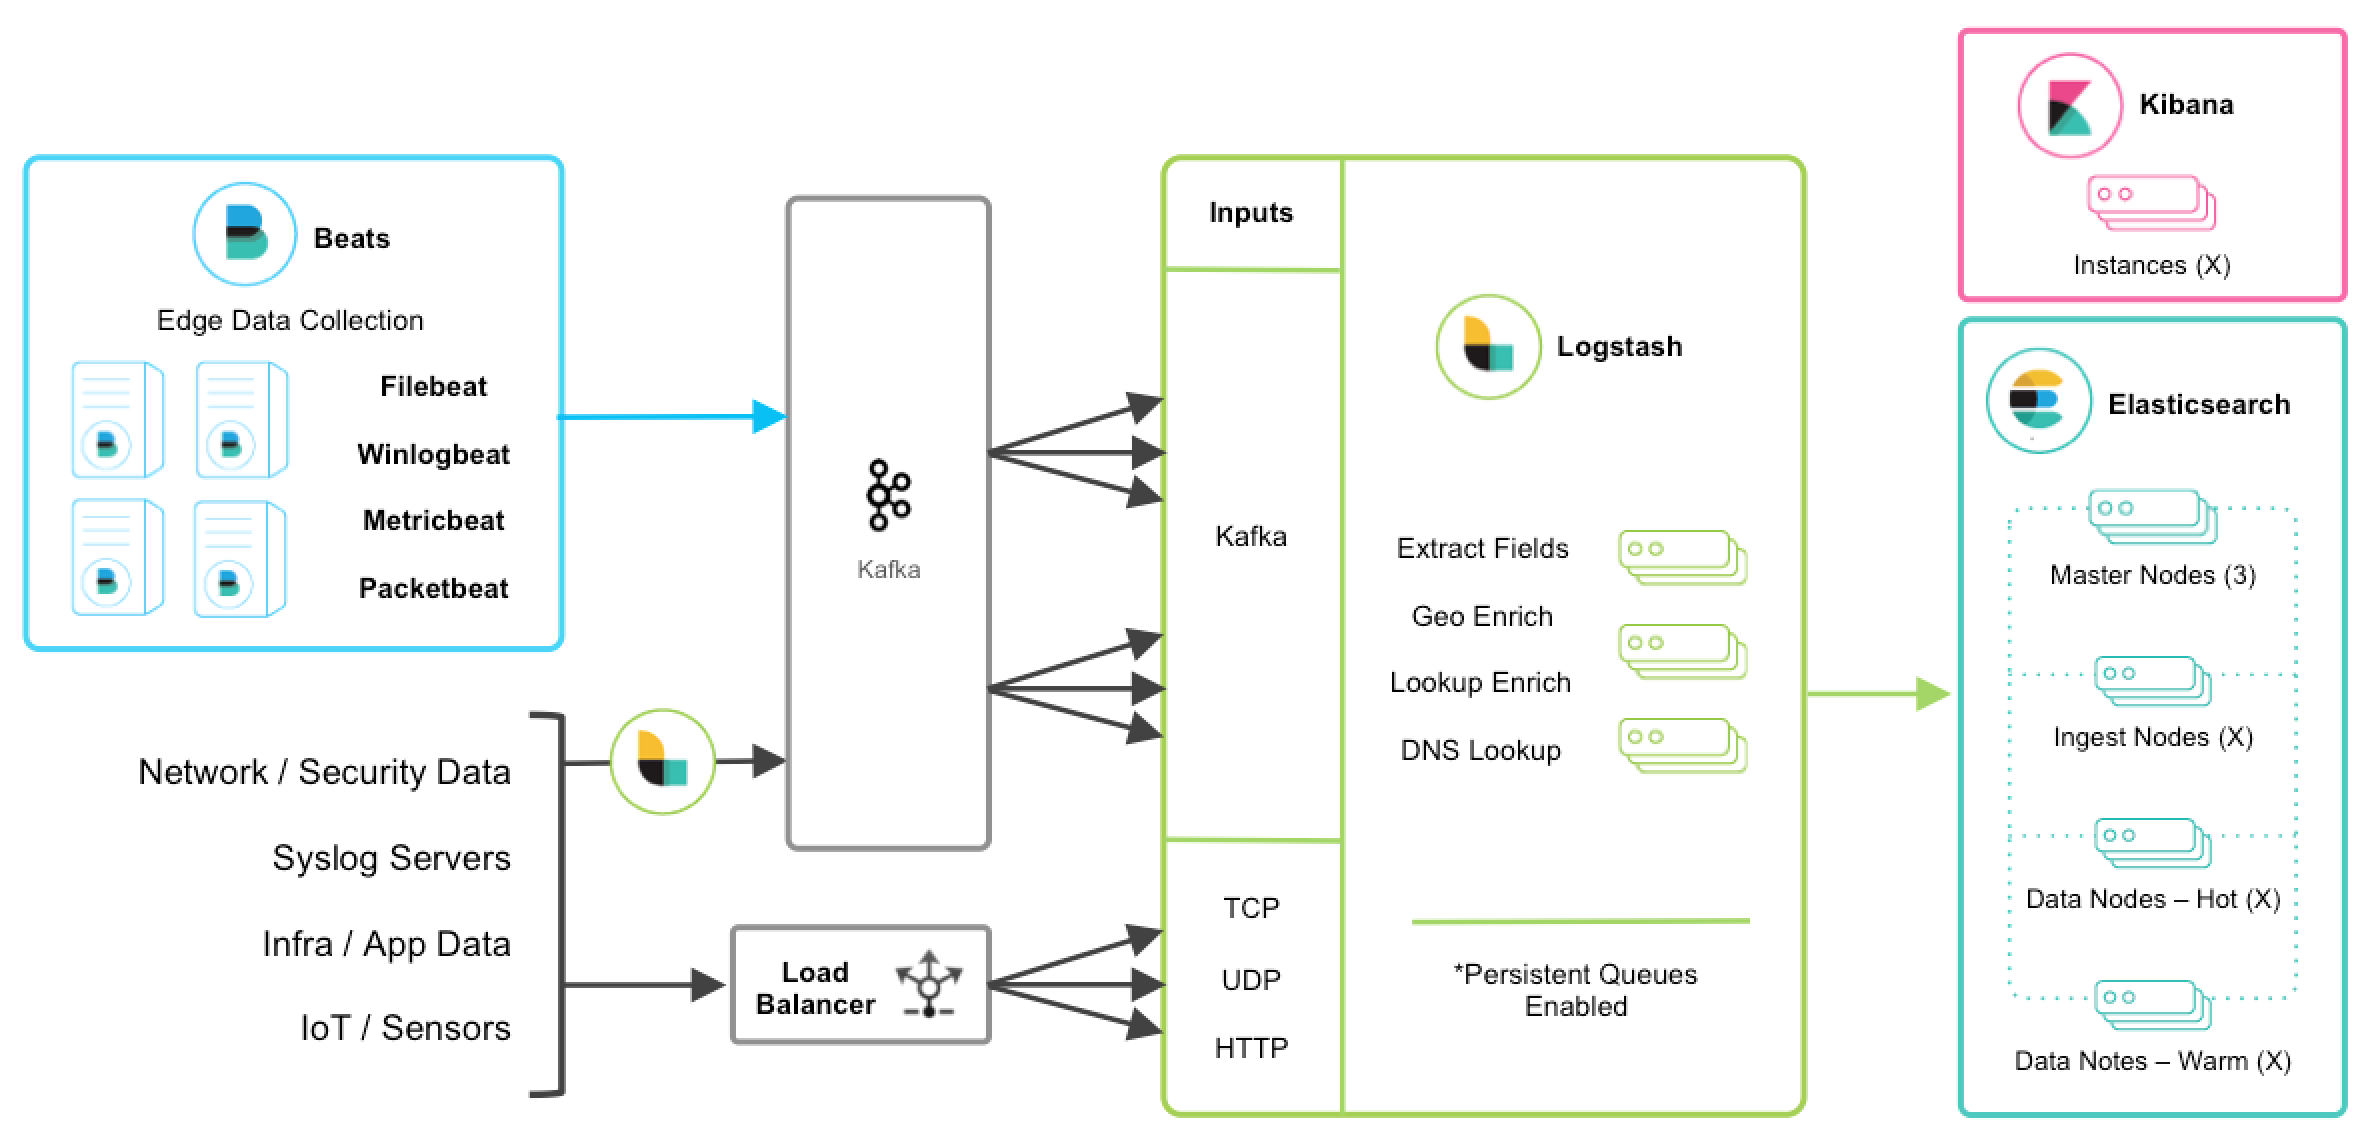
\includegraphics[width=1\textwidth]{mahi/bi-5.png}
\centering
\caption{معماری سیستم مانیتورینگ با استفاده از ELK}
\label{fig:bi-5}
\end{figure}

\subsection{دریافت داده ها}
در ابتدا به بررسی ورودی های سیستم و نحوه گرفتن هر دیتا میپردازیم.
انواع ورودی ها و نرم‌افزار های آن به شرح زیر است.
\begin{enumerate}
    \item دریافت فایل
    \newline
    برای دریافت لاگ فایل ها از ابزار filebeat استفاده شده است تا با نظرات بر مسیر های لاگ ها به محض اضافه شدن خط های لاگ به هر کدام از فایل ها تنها تغییرات آن ها را به سمت صف داده ها منتقل کند.
    \item دریافت وضعیت سیستم
    \newline
    وضعیت سیستم شامل میزان استفاده از پردازنده، حافظه، شبکه به تفکیک نرم‌افزار ها و کاربر های میشود.
    نرم‌افزار metricbeat برای این منظور راه اندازی شده است.
    \item دریافت و کنترل پکت های شبکه
    \newline
    الگو های ارسال و دریافت پکت ها در شبکه و همچنین حجم و نحوه انتقال آن ها از جمله مهم ترین مسائل در سیستم های توزیع شده است. مانیتورینگ و پیدا کردن ناهنچاری در این الگو ها میتواند نشان دهنده خطا های جدی و یا مشکلات امنیتی باشد که باید با دقت بالا نظارت شود. نرم‌افزار packetbeat برای این منظور راه اندازی شده است.
    \item دریافت تغییرات بر روی سیستم عامل و Audit
    \newline
    تغییرات در کانفیگ فایل های سیستم عامل ممکن است تاثیر زیادی بر روی عملکرد نرم‌افزار ها بگذارد، نظارت بر این تغییرات بسیار مهم است.
    این فایل ها با نرم‌افزار Auditbeat یا Winlogbeat کنترل میشود.
    \item دریافت اطلاعات از پایگاه داده
    \newline
    بخش مهمی از اطلاعات بر روی پایگاه های داده ذخیره سازی و گزارش میشود برای دریافت این اطلاعات از پایگاه داده اتصال مستفیم با Oracle توسط JDBC انجام شده است و خروجی کوئری های اجرا شده به صورت Json وارد سیستم میشود.
    این فعالیت بر روی نرم‌افزار Logstash پیاده سازی شده است و کنترل و فیلترینگ اولیه در همان نرم‌افزار پیاده سازی شده است.
    
    \item دریافت از طریق API نرم‌افزارها
    \newline
    نرم‌افزار ها گزارش دهی و داشبور های متفاوتی به سیستم و لایه آنالیز متصل میشود برای ارتباط با این نرم‌افزار ها باید ردخواست ها بر روی پورت HTTPو با API آن نرم‌افزار صورت گیرد که برای نمونه نرم‌افزار Grafana, Tableau, Kibana, OBIEE از این طریق به سیستم متصل هستند.
    این ارتباط نیز بر روی نرم‌افزار Logstash پیاده سازی شده است.
    \item دریافت مستقیم از شبکه
    \newline
    در سیستم هایی که امکان نصب نرم‌افزار به صورت مستقیم برای ما وجود ندارد باید اطلاعات را نتها از طریق شبکه به صورت منظم انتقال دهیم و در سمت دیگر دریافت و پردازش کنیم.
    این عملکرد نیز بر روی Logstash پیاده سازی شده است و برای ارتباط محدود با سرور های خارجی استفاده میشود.
\end{enumerate}

\subsection{صف و نگه داری موقت}

بعد از دریافت ورودی های باید ابتدا آنها را ذخیره و سپس ساختار دهی کرد تا برای استفاده و تحیلی مناسب باشند.
از آنجا که کار ساختار دهی ممکن است زمان بر باشد و با همان سرعت ورودی نتواند صورت گیرد باید یک صف در میان ورودی ها و نرم‌افزار های ساختار دهی قرار گیرد تا از نابودی داده ها جلوگیری کند.

دو نرم‌افزار صف برای ایجاد صف سریع و صف قابل اطمینان در این نرم‌افزار استفاده شده است.

\begin{enumerate}
    \item Kafka (صف قابل اطمینان)
    \newline
    این نرم‌افزار داده ها را بر روی هارد دیسک ذخیره میکند و به صورت توزیع شده در تمامی سیستم ها وجود دارد تمامی داده های ورودی که به صورت Stream ویا در Batch فایل های کوچک دریافت میشود در این سیستم ذخیره میشود زیرا در صورت از بین رفتن آنها نسخه دیگری وجود نخواهد داشت.
    معماری این صف به نحوه ای طراحی شده است تا به سرعت بالا از هارد دیسک استفاده کند و در صورت نیاز چندین پردازش گر به طور موازی اطلاعات را از صف دریافت کرده و پردازش کنند.
    برای ایجاد هماهنگی بین نرم‌افزار های توزیع شده بر روی سرور ها برنامه Zookeeper نیز به صورت توزیع یافته بر روی سیستم ها قرار دارد.
    Zookeeper با معماری masterless کار میکند و در صورت از کار افتادن هر سیستم بقیه سیستم با مشکلی رو به رو نمیشود.
    همچنین صف Kafka حداقل ۳ نسخه از هر داده را سیستم های مختلف ذخیره میکند تا با از دسترس خارج شدن هر سیستم هیچ داده ای از دسترسی خارج نشود.
    \item Redis (صف سریع)
    \newline
    این صف برای ارتباط با سرور هایی که فایل ها را به صورت Batch با حجم بزرگ به ورودی میدهند استفاده شده است و خیلی سریع تنها بر روی حافظه نوشته و خوانده میشود.
    این صف در حقیقت به عنوان یک کش برای سیستم در نظر گرفته شده است تا دسترسی به داده های سنگین را سریع تر کند و نیاز به ارتباط مجدد با سرور ها و انتقال مجدد فایل نباشد.
\end{enumerate}

\subsection{پردازش اولیه و ساختار دهی}
اکثر داده های دریافتی این سیستم بدون ساختار و برای جستجو و تحلیل مناسب نیستند، بنابراین باید در مرحله اول به داده ها ساختار داد و اطلاعات نامعتبر را حذف کرد.
نرم افزار Logstash به صورت توزیع شده در سرور ها در حال کار است و اطلاعات را از منابع و یا صف ها میگیرد.
این اطلاعات با فیلتر های متفاوت و الگو ها مشخص شده ساختار میگیرند و برای پردازش آماده میشود.
از جمله فیلتر ها مورد استفاده میتوان به موارد زیر اشاره کرد.
\begin{enumerate}
    \item GROK
    \newline 
    این فیلتر به کمک الگو ها بسیار زیادی که به صورت اپن سورس وجود دارد یکی از قدرتمند ترین ابزار های ساختار دهی اطلاعات است که در اکثر مواقع مورد استفاده قرار میگیرد.
    \item RegExp
    \newline 
    این فیلتر مانند regular expression در دیگر زبان ها و ابزار قادر به تفکیک و تشخیص الگو ها تا حد regex میباشد.
    \item Ruby
    \newline
    در حقیقت ruby یک زبان برنامه نویسی است که در اینجا میتوان از آن به عنوان یک فیلتر به صورت مستفیم استفاده کرد.
    \item Standard Format
    \newline
    همچنین فیلتر های بسیار زیادی برای فرمت های استاندارد وجود دارد از جمله CSV, Json, XMLو همچنین قابلیت جداسازی داده ها بر روی پروتکل های معروف مانند HTTP, TCP, UDP, JDBC, ...
\end{enumerate}

در پایان خروجی این بخش به صورت داده های Jsonبرای موتور جستجو  Elastic ارسال میشود که به صورت توزیع شده در تمامی سرور ها قرار دارد.

\subsection{نگه داری داده ها و موتور جستجو}
موتور جستجو Elasticsearch به عنوان پایگاه داده NoSQL برای نگه داری طولانی مدت داده ها و اعمال تحلیل استفاده میشود از آنجا که این یک موتور جستجو است برای پردازش داده ها و ایجاد تغییر در آنها بسیار مناسب نبوده اما سرعت بالایی در دریافت، ایندکس و جستجو اطلاعات دارد.
از این رو به یک سیستم پردازشی در کنار Elastic برای تحلیل اطلاعات و ایجاد ارتباط و محاسبات نیاز داریم.
با توجه به اینکه داده ها خروجی سیستم ها و گزارش آنها هستند در حقیقت پردازش شده میباشند و بار پردازشی بالایی نیاز نیست و اعمال توابع جمع بندی و نتیجه گیری مورد استفاده قرار میگیرد.

\subsection{تحلیل داده ها}
از آنجا که داده ها به صورت توزیع شده در موتور جستجو هستند تحلیل آنها نیز میتواند به صورت توزیع شده انجام شود و به کمک الگوریتم های Map و Reduce این تحلیل ها صورت گیرد.

برنامه Spark برای این منظور به صورت توزیع شده در تمامی سرور ها نصب و راه اندازی شده است و عملیات دریافت داده ها پردازش و لود دوباره داده ها در elasticبا این برنامه صورت میگیرد.

همچنین برای مدیریت cluster برنامه Spark از نرم‌افزار Mesos استفاده شده است تا بار و کار تعریف شده را بین تمامی نود های این خوشه تقسیم کند و در نهایت نتایج را به Elastic ارسال کند.

تحلیل های صورت گرفته در این سیستم به صورت بدون ناظر Unsupervised انجام شده است و عبارت است از:
\begin{enumerate}
    \item تشخیص ناهنجاری ها
    \newline
    با پیدا کردن الگو های رفتاری هر پارامتر در هر ساعت از شبانه روز و یا روز هفته میتوان به رفتار هایی که اختلاف زیادی با الگو دارد به راحتی پی برد.
    وجود چنین رفتار هایی به طور کلی یا باید از تغییر آگانه در سیستم رخ داده باشد و یا خطایی در بخشی ایجاد شده است.
    در هر دوصورت نظارت بر این تغییرات و اندازه گیری آنها کمک بسیاری به خطا یابی و یا بهینه سازی عملکرد سیستم میکند.
    \item خوشه بندی رفتار ها سیستم
    \newline
    خوشه بندی رفتاری سیستم کمک میکند که سیستم را بهتر بشناسیم و با توجه به هر حالت سیستم تصمیم گیری شود.
    برای مثال در حالت هایی که بار بسیار زیادی در استفاده از پردازنده است سیستم حافظه کش بیشتری در اختیار نرم‌افزار ها میدهد تا فشار کمتر شود و در حالت هایی فشار بر روی حافظه بیشتر از فعالیت های موازی بیشتری انجام دهد و از پردازنده استفاده بیشتری کند تا سیستم را به تعادل برساند.
    \item پیش بینی وضعیت سیستم
    \newline
    پیشگیری از وقوع خطا و مشکل در سیستم بسیار موثر تر از گزارش خطا و کمک در رفع آن است بنابراین سیستم پیش بینی وضعیت سیستم با توجه به الگو های قبلی میتواند قبل از رقوع رخداد وجود آن را به تیم اطلاع دهد و تیم اقدام به جلوگیری از بروز خطا کند.
\end{enumerate}

\subsection{نمایش و استفاده از داده ها}
در نهایت باید سیستم بتواند خروجی این تحلیل ها و داده ها رو به صورت واضحی برای کاربران نمایش دهد و همچنین در صورت نیاز از طریق کانال های ارتباطی به آنها اطلاع دهد.
از این رو سیستم های زیر در بخش های مختلف مورد استفاده قرار گرفته است.
\begin{enumerate}
    \item Kibana
    \newline
    برای مدیریت و کنترل خوشه مانیتورینگ استفاده شده است و کار تعریف و اصلاح ایندکس های موتور جستجو در این نرم‌افزار صورت میگیرد.
    در این نرم‌افزار میتوان گزارش های ساده ای را گرفت و به صورت کلی نمایی از داده ها را داشت اما به صورت تخصصی برای این کار ساخته نشده است.
    \item Grafana
    \newline
    این نرم‌افزار برای تولید گراف ها و تصاویر گویا از وضعیت سیستم است که به طور کلی برای نمایش خروجی تمامی گزارش ها استفاده میشود.
    \item Alert Manager
    \newline
    این ابزار برای ارسال پیام در برنامه های مختلف در صورت بروز مشکل استفاده شده است.
    راه های ارتباطی مورد استفاده در حال حاضر برای این سیستم ایمیل، پیامک، JIRAو Telegram می‌باشد.
\end{enumerate}

\subsection{مدیریت سرور ها و نیازمندی های جدید}
با توجه به معماری توزیع شده این نرم‌افزار و تعداد زیاد سرور های ایجاد تغییرات در این سیستم به شدت زمان بر و پرخطااست.
و همچنین راه اندازی سرور های جدید نیاز به زمان و فعالیت زیادی دارد تا با بقیه سیستم یکپارچه شود.

برای حل این مشکل راه کاری های مدیریت نتظیمات و راه اندازی خودکار باید مورد استفاده قرار گیرد.
محصولی که به این عتوان در این پروژه استفاده شده است Redhat Ansible است.
به کمک Ansible ایجاد تغییرات دیگر تنها یکبار صورت میگیرد و در دیگر سیستم ها اعمال میشود و سرعت کار بسیار بالا تر است و احتمال خطا به شدت پایین تر، از سوی دیگر نصب و راه اندازی نرم‌افزار ها به صورت یکپارچه و مشترک از طریق Ansible صورت میگیرد.

علت انتخاب Ansible نسبت به دیگر ابزار های موجود تفاوت اصلی آن در معماری برنامه است. معماری Ansible بدون نیاز به نصب در سرور های مقصد و یا داشتن یه سرویس به صورت مداوم در کنار پروژه است. Ansible فقط در صورت نیاز و اعمال تغییر اجرا میشود و پس از انجام تسک ها تعریف شده برنامه پایان می‌یابد و از طریق پروتکل ssh با سرور ها در ارتباط است و تمامی تنظیمات و تغییرات به صورت شفاف قابل مشاهده است.


\section{نتیچه گیری}
در این پروژه یک سیستم مانیتورینگ قابل اطمینان با بازدهی بالا برای نظارت و کنترل بلادرنگ پروژه هوش تجاری شرکت مخابرات همراه اول توصیف شد و انواع راه حل ها و مراحل اجرا آن تشریح گردید.

با توجه به اهمیت روز افزون داده و استفاده از علوم داده برای بالا بردن کیفیت محصولات نیازمندی های جدید به پردازش سریعتر و قابل اطمینان تر ایجاد میشود. در این پروژه سعی شده است تا با یک سیستم توزیع شده تضمین در درسترس بودن و اطمینان از سیستم حاصل گردد و سرعت پردازش با استفاده از روش های پردازش موازی و توزیع شده افزایش یابد. لازم به ذکر است هزینه توسعه و تغییر این سیستم و حتی تعمیرات به شدت کمتر از یک سیستم با چنین توانایی است وزمان راه اندازی و توسعه بسیار کمتر و فرآیند ساده تر می‌باشد.

\section{کار های آینده}

این پروژه به بررسی گزارش ها و داده های سیستمی و پردازش آنها به صورت غیرناظر پرداخته است. از جمله فعالیت های قابل اجرا در آینده پروژه افزودن تحلیل داده های تجاری و همچنین نظارت بر تیم توسعه و فعالیت های HR بر این سیستم است.

از جمله توسعه های فنی در این حوزه میتوان به انتقال داده ها بر روی Hadoop اشاره کرد تا توزیع سیستم در لایه فایل سیستم نیز صورت گیرد.

\end{document}
